%
% NOTE -- ONLY EDIT THE .Rnw FILE!!!  The .tex file is
% likely to be overwritten.
%
% \VignetteIndexEntry{Metabolite Identification with MetFrag in R}
% \VignetteKeywords{mass spectrometry, tandemms, metabolite identification}
% \VignettePackage{metfRag}
\documentclass[12pt, a4paper]{scrartcl}\usepackage[]{graphicx}\usepackage[]{color}
%% maxwidth is the original width if it is less than linewidth
%% otherwise use linewidth (to make sure the graphics do not exceed the margin)
\makeatletter
\def\maxwidth{ %
  \ifdim\Gin@nat@width>\linewidth
    \linewidth
  \else
    \Gin@nat@width
  \fi
}
\makeatother

\definecolor{fgcolor}{rgb}{0.345, 0.345, 0.345}
\newcommand{\hlnum}[1]{\textcolor[rgb]{0.686,0.059,0.569}{#1}}%
\newcommand{\hlstr}[1]{\textcolor[rgb]{0.192,0.494,0.8}{#1}}%
\newcommand{\hlcom}[1]{\textcolor[rgb]{0.678,0.584,0.686}{\textit{#1}}}%
\newcommand{\hlopt}[1]{\textcolor[rgb]{0,0,0}{#1}}%
\newcommand{\hlstd}[1]{\textcolor[rgb]{0.345,0.345,0.345}{#1}}%
\newcommand{\hlkwa}[1]{\textcolor[rgb]{0.161,0.373,0.58}{\textbf{#1}}}%
\newcommand{\hlkwb}[1]{\textcolor[rgb]{0.69,0.353,0.396}{#1}}%
\newcommand{\hlkwc}[1]{\textcolor[rgb]{0.333,0.667,0.333}{#1}}%
\newcommand{\hlkwd}[1]{\textcolor[rgb]{0.737,0.353,0.396}{\textbf{#1}}}%

\usepackage{framed}
\makeatletter
\newenvironment{kframe}{%
 \def\at@end@of@kframe{}%
 \ifinner\ifhmode%
  \def\at@end@of@kframe{\end{minipage}}%
  \begin{minipage}{\columnwidth}%
 \fi\fi%
 \def\FrameCommand##1{\hskip\@totalleftmargin \hskip-\fboxsep
 \colorbox{shadecolor}{##1}\hskip-\fboxsep
     % There is no \\@totalrightmargin, so:
     \hskip-\linewidth \hskip-\@totalleftmargin \hskip\columnwidth}%
 \MakeFramed {\advance\hsize-\width
   \@totalleftmargin\z@ \linewidth\hsize
   \@setminipage}}%
 {\par\unskip\endMakeFramed%
 \at@end@of@kframe}
\makeatother

\definecolor{shadecolor}{rgb}{.97, .97, .97}
\definecolor{messagecolor}{rgb}{0, 0, 0}
\definecolor{warningcolor}{rgb}{1, 0, 1}
\definecolor{errorcolor}{rgb}{1, 0, 0}
\newenvironment{knitrout}{}{} % an empty environment to be redefined in TeX

\usepackage{alltt}

%Neue Pakete
\usepackage[latin1]{inputenc}
\usepackage[T1]{fontenc}
\usepackage[ngerman]{babel}
\usepackage[backend=bibtex, sorting=none]{biblatex}
\usepackage{hyperref}
\usepackage{graphicx}
\usepackage{pdfpages}

\usepackage{csquotes}
\usepackage{amsmath}
\usepackage{amsfonts}
\usepackage{amssymb}

\usepackage{tikz}
\usetikzlibrary{positioning,shapes,backgrounds}

\usepackage[a4paper,left=5cm,right=1cm,top=2cm,bottom=2cm]{geometry}
\usepackage{fullpage}
\setlength{\headsep}{1em}
\setlength{\parindent}{0em}
\setlength{\headheight}{13.87178pt}

\renewcaptionname{ngerman}{\contentsname}{Table of Contents}
\renewcaptionname{ngerman}{\listfigurename}{Figures}
\renewcaptionname{ngerman}{\listtablename}{Tables}
\renewcaptionname{ngerman}{\figurename}{Figure}
\renewcaptionname{ngerman}{\tablename}{Table}

\newcommand{\Robject}[1]{{\texttt{#1}}}
\newcommand{\Rfunction}[1]{{\texttt{#1}}}
\newcommand{\Rpackage}[1]{{\textit{#1}}}
\newcommand{\Rclass}[1]{{\textit{#1}}}
\newcommand{\Rmethod}[1]{{\textit{#1}}}
\newcommand{\Rfunarg}[1]{{\textit{#1}}}

\bibliography{references.bib}
\IfFileExists{upquote.sty}{\usepackage{upquote}}{}
\begin{document}
%\SweaveOpts{concordance=TRUE}
\title{Metabolite Identification with MetFrag in R}
\author{C. Ruttkies, S. Neumann, A. Helmchen}
\maketitle

\newpage
\tableofcontents

\newpage
\section{Introduction}
In this section the MetFragR package is introduced and described.
For a better understanding the functionality of a mass spectrometer (MS/MS) was outlined. 
Initially, the package shall be loaded.

\begin{knitrout}
\definecolor{shadecolor}{rgb}{0.969, 0.969, 0.969}\color{fgcolor}\begin{kframe}
\begin{alltt}
\hlkwd{library}\hlstd{(rcdk)}
\hlkwd{library}\hlstd{(metfRag)}
\end{alltt}
\end{kframe}
\end{knitrout}

For the understanding of the metabolism of several organisms different analysis methods
are necessary. One of these methods is referred as mass spectrometry to detect and identify compounds 
in samples \cite{Dunn2008}. These compounds are partially unknown and have to be determined and annotated
to understand other metabolic circles and pathways. On the other hand mass spectrometry can help to 
identify known proteins or posttranslational modifications (PTMs) like alteration caused by phosphate. \\[0.5em]
Actually, to obtain applicable results of an unknown molecule tandem mass spectrometry MS/MS or \(\text{MS}^\text{2}\) 
is used, because additional structural hints and the exact mass of fragments of a compound are delivered \cite{Wolf2010}.
Hence, two mass spectrometers are combined. In the first MS based on a given mass a single precursor ion is selected. 
The molecule is colliding with a neutral gas (collision-induced dissociation (CID)). This compound is then cleaved into
several fragments which can be distinguished by a given mass \cite{Jeol2006}. \\[0.5em]
This results in a MS/MS spectrum which contains only product ions from selected precursor ion. 
The spectra indicate the mass-to-charge ratio (m/z ratio) which used by the MS/MS to deflect specific ions to the analysator. 
The ion detector data produce a fragmentation spectrum with the m/z ratio against the abundance of each compound. \\[0.5em]
Hence, to use the statistical power of R we write the package \Rpackage{metfRag} which expand the features of 
MetFrag by the capabilities of R. Metfrag performs an in silico refragmentation of compounds. 
Therefor, compound libraries are compared with spectra of unknown metabolites \cite{Wolf2010}.
Metfrag is written in Java so that it was integrated in metfRag by using \Rpackage{rJava} \cite{Urbanek2013}
The package 'metfRag' uses the precursor mass, the compound id or the formula to obtain a candidate list of compounds 
from KEGG or PubChem. Additionally, it provides functions to process the obtained candidate list and calculates ranking parameters
like the optimistic, the pessimistic or the relative rank.

\newpage
\section{Methods of the MetFragR package}
In this section the functions of this package are described. Firstly, the loading of compounds
and the processing are explained. Then a ranking procedure is introduced to generate own ranking methods by
using own properties or functions. Additionally, an example illustrates the functional principle
on mentioned methods. 
\subsection{Structure file preparation}
To load compounds from a chemical table file like SDF you can directly use the 
function from \Rpackage{rcdk}. In the example below a metfRag system file is used. The included SDF 
is the result of MetFusion processing of the MS/MS spectrum of the CASMI 2014 challenge 5 \cite{Guha2007}.
\begin{knitrout}
\definecolor{shadecolor}{rgb}{0.969, 0.969, 0.969}\color{fgcolor}\begin{kframe}
\begin{alltt}
\hlstd{file} \hlkwb{<-} \hlstr{"sdf/metfusion-category2-Challenge5-pubchem.sdf"}
\hlstd{sdfile} \hlkwb{<-} \hlkwd{system.file}\hlstd{(file,} \hlkwc{package} \hlstd{=} \hlstr{"metfRag"}\hlstd{)}
\hlstd{mols} \hlkwb{<-} \hlkwd{load.molecules}\hlstd{(sdfile)}
\end{alltt}
\end{kframe}
\end{knitrout}
\subsection{Getting compounds from a database}
To get a list of molecules without a file we send a query to available 
databases KEGG or PubChem by using the exact mass and the mass deviation (in ppm) to specify a compound. In addition to that, metfRag uses RCurl to retrieve the results which delivers a database \cite{Lang2013a}.
Additionally, metfRag can be used to search by a database identifier/ID. KEGG uses three parameters among them also the mol weight. Let us view an example for PubChem to get some molecules but the same could be applied for KEGG:

\begin{knitrout}
\definecolor{shadecolor}{rgb}{0.969, 0.969, 0.969}\color{fgcolor}\begin{kframe}
\begin{alltt}
\hlstd{params} \hlkwb{<-} \hlkwd{list}\hlstd{(}\hlkwc{mass}\hlstd{=}\hlnum{174.05}\hlstd{,} \hlkwc{range}\hlstd{=}\hlnum{0.001}\hlstd{);}
\hlstd{pubchem.mol} \hlkwb{<-} \hlkwd{db.pubchem.getId}\hlstd{(params)[}\hlnum{1}\hlopt{:}\hlnum{5}\hlstd{,];}
\hlstd{pubchem.mol[}\hlnum{1}\hlopt{:}\hlnum{5}\hlstd{]}
\end{alltt}
\begin{verbatim}
## [[1]]
## [1] "84766583"
## 
## [[2]]
## [1] "84654828"
## 
## [[3]]
## [1] "84654827"
## 
## [[4]]
## [1] "84654826"
## 
## [[5]]
## [1] "84654825"
\end{verbatim}
\end{kframe}
\end{knitrout}

Each entry of the result is converted to an IAtomContainer which is described in the manual from 
\Rpackage{rcdk} \cite{Guha2007}. Every container contains properties which can be altered by an user. If one send a request, PubChem add specific properties like IUPAC name and deliver the associated molecules. This information is necessary to process the molecules further with set operations. \\[0.5em]
KEGG use the Representational State Transfer (REST) paradigma to grant web access to own data. Therefor, metfRag use the package KEGGREST from Bioconductor \cite{Tenenbaum}. Hence, each query and the obtained additional properties build two requests. \\[0.5em]
Similarly, metfRag use for the PubChem requests the paradigma PUG REST (power user gateway) which apply FTP to give a access to the data \cite{Southern2011}. To obtain the results in a structured form metfRag uses XML to process the resulted XML files to IAtomContainer \cite{Lang2013b}. The number of candidates is limited by PubChem and metfRag to default value 100.

\begin{knitrout}
\definecolor{shadecolor}{rgb}{0.969, 0.969, 0.969}\color{fgcolor}\begin{kframe}
\begin{alltt}
  \hlstd{pubchem.container} \hlkwb{<-} \hlkwd{db.pubchem.getMoleculeContainer}\hlstd{(pubchem.mol)}
  \hlkwd{get.properties}\hlstd{(pubchem.container[[}\hlnum{1}\hlstd{]])[}\hlnum{1}\hlopt{:}\hlnum{5}\hlstd{]}
\end{alltt}
\begin{verbatim}
## $`cdk:Title`
## [1] "84766583"
## 
## $`cdk:Remark`
## [1] NA
## 
## $COMPOUND_CID
## [1] "84766583"
## 
## $COMPOUND_CANONICALIZED
## [1] "1"
## 
## $CACTVS_COMPLEXITY
## [1] "143"
\end{verbatim}
\end{kframe}
\end{knitrout}

\newpage
\subsection{Union, intersect and build difference of compounds}
To perform set operations on IAtomContainers two compound lists are necessary. The operation occurs by using molecule 
properties which are equal in both container lists. 
Thereto, the database prefix from each molecule property was removed. To adept the equal properties we could omit the third link parameter or we call the function \Rfunction{showLinkOptions}.

\begin{knitrout}
\definecolor{shadecolor}{rgb}{0.969, 0.969, 0.969}\color{fgcolor}\begin{kframe}
\begin{alltt}
  \hlstd{opt} \hlkwb{<-} \hlkwd{container.union}\hlstd{(pubchem.container,pubchem.container)}
\end{alltt}
\begin{verbatim}
## NULL
\end{verbatim}


{\ttfamily\noindent\color{warningcolor}{\#\# Warning: Please choose a link from above. You could use the\\\#\#\ \ \ \ \ \ \ \ \ \ function: comm.lib.showLinkOptions(set.a,set.b)}}\end{kframe}
\end{knitrout}

This show us the possible links of both container. To union the both sets we could call \Rfunction{container.union} and \Rfunction{container.intersect} to intersect two container sets. Then, the molecule property from first list was compared with each molecule property from second list. The doubled occurence of an element are filtered which means that the 
first element is in the list and the second element is discard.

\begin{knitrout}
\definecolor{shadecolor}{rgb}{0.969, 0.969, 0.969}\color{fgcolor}\begin{kframe}
\begin{alltt}
  \hlkwd{container.union}\hlstd{(pubchem.container,}
                  \hlstd{pubchem.container,}
                  \hlstr{"MOLECULAR_FORMULA"}\hlstd{)}

  \hlkwd{container.intersect}\hlstd{(pubchem.container,}
                      \hlstd{pubchem.container,}
                      \hlstr{"MOLECULAR_FORMULA"}\hlstd{)}
\end{alltt}
\end{kframe}
\end{knitrout}

If we would like to build the symmetric difference or asymmetric difference we could call \Rfunction{container.symmetric.difference} and \Rfunction{container.asymmetric.difference}. 

\begin{knitrout}
\definecolor{shadecolor}{rgb}{0.969, 0.969, 0.969}\color{fgcolor}\begin{kframe}
\begin{alltt}
  \hlkwd{container.symmetric.difference}\hlstd{(pubchem.container,}
                                 \hlstd{pubchem.container,}
                                 \hlstr{"MOLECULAR_FORMULA"}\hlstd{)}

  \hlkwd{container.asymmetric.difference}\hlstd{(pubchem.container,}
                                 \hlstd{pubchem.container,}
                                 \hlstr{"MOLECULAR_FORMULA"}\hlstd{)}
\end{alltt}
\end{kframe}
\end{knitrout}

We could search a molecule by a link in a list of compounds. At that point we are interested in all positions where
the molecule occurs. 
Thereto, we call the function \Rfunction{common.lib.lookup}. The link describes a property of the molecule. The value of a given molecule is validated against the properties in the compound list. To split a property like 'IUPAC\_INCHIKEY' into parts the parameter 'split' is introduced. This parameter is a list with a seperator and the position of the substring which is used for the comparison.

\begin{knitrout}
\definecolor{shadecolor}{rgb}{0.969, 0.969, 0.969}\color{fgcolor}\begin{kframe}
\begin{alltt}
  \hlstd{split} \hlkwb{<-} \hlkwd{list}\hlstd{(}\hlkwc{sep}\hlstd{=}\hlstr{"-"}\hlstd{,} \hlkwc{pos}\hlstd{=}\hlnum{3}\hlstd{)}
  \hlkwd{common.lib.lookup}\hlstd{(pubchem.container[[}\hlnum{1}\hlstd{]],}
                    \hlstd{pubchem.container,}
                    \hlstr{"IUPAC_INCHIKEY"}\hlstd{,}
                    \hlstd{split)}
\end{alltt}
\begin{verbatim}
## [1] 1 2 3 4 5
\end{verbatim}
\end{kframe}
\end{knitrout}

Another variant of this principle is the function \Rfunction{common.lib.lookupFirst}. Only the first occurence of a molecule is considered.

\begin{knitrout}
\definecolor{shadecolor}{rgb}{0.969, 0.969, 0.969}\color{fgcolor}\begin{kframe}
\begin{alltt}
  \hlstd{split} \hlkwb{<-} \hlkwd{list}\hlstd{(}\hlkwc{sep}\hlstd{=}\hlstr{"-"}\hlstd{,} \hlkwc{pos}\hlstd{=}\hlnum{3}\hlstd{)}
  \hlkwd{common.lib.lookupFirst}\hlstd{(kegg.container[[}\hlnum{1}\hlstd{]],}
                         \hlstd{pubchem.container,}
                         \hlstr{"IUPAC_INCHIKEY"}\hlstd{,}
                         \hlstd{split)}
\end{alltt}
\end{kframe}
\end{knitrout}

\newpage
\subsection{Scoring structures with MetFrag}
To score received compounds from a database MetFragR uses two options. On the one hand scoring of a chemical table format SDF or mol file. For this option metfRag needs a path. Obligatory this package needs the mass-to-charge ratio values from the peak list, the intensity values and the exact mass of the 
precursor ion. 

\begin{knitrout}
\definecolor{shadecolor}{rgb}{0.969, 0.969, 0.969}\color{fgcolor}\begin{kframe}
\begin{alltt}
\hlstd{file} \hlkwb{<-} \hlstr{"sdf/metfusion-category2-Challenge5.mf"}
\hlstd{queryfile} \hlkwb{<-} \hlkwd{system.file}\hlstd{(file,} \hlkwc{package} \hlstd{=} \hlstr{"metfRag"}\hlstd{)}
\hlstd{challenge5} \hlkwb{<-} \hlkwd{read.table}\hlstd{(queryfile,}
                         \hlkwc{sep}\hlstd{=}\hlstr{"\textbackslash{}t"}\hlstd{,}
                         \hlkwc{col.names}\hlstd{=}\hlkwd{c}\hlstd{(}\hlstr{"mz"}\hlstd{,} \hlstr{"inten"}\hlstd{))}

\hlstd{scoredMols} \hlkwb{<-} \hlkwd{score.molecules.from.sdf}\hlstd{(sdfile,}
                                       \hlkwc{mzs}\hlstd{=challenge5[,}\hlstr{"mz"}\hlstd{],}
                                       \hlkwc{ints}\hlstd{=challenge5[,}\hlstr{"mz"}\hlstd{],}
                                       \hlkwc{exact.mass}\hlstd{=}\hlnum{290.0646}\hlstd{,}
                                       \hlkwc{mz.abs}\hlstd{=}\hlnum{0.001}\hlstd{,}
                                       \hlkwc{mz.ppm}\hlstd{=}\hlnum{5}\hlstd{,}
                                       \hlkwc{search.ppm}\hlstd{=}\hlnum{5}\hlstd{,}
                                       \hlkwc{pos.charge}\hlstd{=}\hlnum{TRUE}\hlstd{,}
                                       \hlkwc{mode}\hlstd{=}\hlnum{1}\hlstd{,}
                                       \hlkwc{tree.depth}\hlstd{=}\hlnum{2}\hlstd{)}
\hlstd{scoredMols} \hlkwb{<-} \hlstd{mols}
\end{alltt}
\end{kframe}
\end{knitrout}

These example values are extracted from the MetFrag Website \cite{Metfrag2014}. A MS/MS spectrum was generated by using the entered parameters (Figure \ref{fragSpec}).
\newpage
\begin{figure}[h]
  \centering
  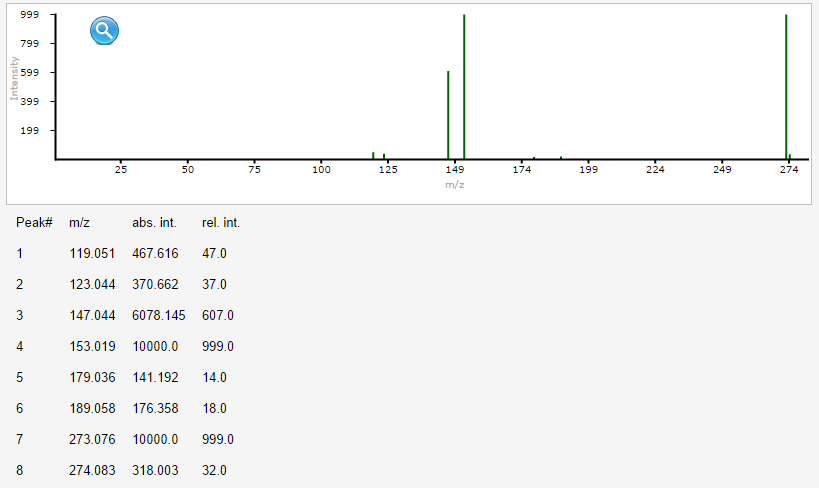
\includegraphics[scale=0.5]{./figure/Metfrag_screenshot.png}
  \caption{MS/MS spectrum of the MetFrag Website with the neutral mass 272.06847 and the example 
  values for each peak. They are characterised by the mass-to-charge values (m/z), the absolute intensities (abs.int)
  and the relative intensities (rel.int).}
  \label{fragSpec}
\end{figure}

On the other hand the molecules can be passed as IAtomContainer list which is loaded by \Rpackage{rcdk}. 
For this reason the optional search.ppm parameter is not necessary. Previously, the compound list could have been
generated with help of the database functions \Rfunction{db.kegg.getMoleculeContainer} or
\Rfunction{db.pubchem.getMoleculeContainer} mentioned before in section 2.2.

\begin{knitrout}
\definecolor{shadecolor}{rgb}{0.969, 0.969, 0.969}\color{fgcolor}\begin{kframe}
\begin{alltt}
  \hlstd{mzs} \hlkwb{<-} \hlkwd{c}\hlstd{(}\hlnum{119.051}\hlstd{,}\hlnum{123.044}\hlstd{,}\hlnum{147.044}\hlstd{,}\hlnum{153.019}\hlstd{,}\hlnum{179.036}\hlstd{,}
           \hlnum{189.058}\hlstd{,}\hlnum{273.076}\hlstd{,}\hlnum{274.083}\hlstd{)}
  \hlstd{ints} \hlkwb{<-}\hlkwd{c}\hlstd{(}\hlnum{467.616}\hlstd{,}\hlnum{370.662}\hlstd{,}\hlnum{6078.145}\hlstd{,}\hlnum{10000.0}\hlstd{,}\hlnum{141.192}\hlstd{,}
           \hlnum{176.358}\hlstd{,}\hlnum{10000.000}\hlstd{,}\hlnum{318.003}\hlstd{)}

  \hlstd{pubchem.container} \hlkwb{<-} \hlkwd{score.molecules.from.container}\hlstd{(}
    \hlstd{pubchem.container,}
    \hlstd{mzs,}
    \hlstd{ints,}
    \hlnum{272.06847}\hlstd{)}
\end{alltt}
\end{kframe}
\end{knitrout}

\newpage
After the scoring seven new scoring properties are added to the database specific properties.

\begin{knitrout}
\definecolor{shadecolor}{rgb}{0.969, 0.969, 0.969}\color{fgcolor}\begin{kframe}
\begin{alltt}
  \hlkwd{tail}\hlstd{(}\hlkwd{get.properties}\hlstd{(pubchem.container[[}\hlnum{1}\hlstd{]]),} \hlkwc{n}\hlstd{=}\hlnum{7}\hlstd{)}
\end{alltt}
\begin{verbatim}
## $MetFragID
## [1] "0"
## 
## $PeakScore
## [1] 922.6
## 
## $BondEnergyScore
## [1] 960
## 
## $Score
## [1] 0.75
## 
## $NoPeaksExplained
## [1] 1
## 
## $Rank
## [1] 1
## 
## $PeaksExplained
## [1] "119.051 47.0 "
\end{verbatim}
\end{kframe}
\end{knitrout}

\newpage
\subsection{Rank molecules among a given function or IAtomContainer properties}
If we want like to rank given molcules we need to specify the ranking parameters.
Accordingly, the values BC (candidates with a better score), WC (candiates
with a worse score), EC (candidates with equal score) and TC (total number of candidates) were introduced. \\[0.5em]
With given parameters we can rank our molecules and determine the optimistic rank (OR), 
the pessimistic rank (PR) and the relative rank (RRP) of a molecule based on the condition \cite{Wolf2010}.
\begin{align*}
  PR &= BC + EC + 1 \\
  OR &= BC + 1 \\
  RRP &= 0.5 \cdot (1-\frac{BC-WC}{TC-1})
\end{align*}
For example we have a list of molecules. These molecules should be ranked 
by numeric molecule properties. To display all numeric properties the function 
\Rfunction{comm.lib.showNumberOptions} could be used. If you call the ranking 
function \Rfunction{scoring.getRanks} without a sorting property the output will be the same.

\begin{knitrout}
\definecolor{shadecolor}{rgb}{0.969, 0.969, 0.969}\color{fgcolor}\begin{kframe}
\begin{alltt}
  \hlkwd{comm.lib.showNumberOptions}\hlstd{(pubchem.container)}
\end{alltt}
\end{kframe}
\end{knitrout}

With this parameter we get the possible sorting parameters by which the compounds are classified. 
In addition to this we need the common condition which we get by using the function 
\Rfunction{comm.lib.showLinkOptions}. As a result the condition list contain a name which determined by molecule property name
and a value which determined by molecule property value. 

\begin{knitrout}
\definecolor{shadecolor}{rgb}{0.969, 0.969, 0.969}\color{fgcolor}\begin{kframe}
\begin{alltt}
  \hlstd{sorting} \hlkwb{<-} \hlkwd{list}\hlstd{(}\hlstr{"PeakScore"}\hlstd{,}\hlstr{"Score"}\hlstd{)}
  \hlstd{condition} \hlkwb{<-} \hlkwd{list}\hlstd{(}\hlkwc{IUPAC_INCHIKEY}\hlstd{=}\hlstr{"PAFJIHSCEHOAMQ-UHFFFAOYSA-N"}\hlstd{)}
  \hlkwd{scoring.getRanks}\hlstd{(pubchem.container, sorting, condition)}
\end{alltt}
\begin{verbatim}
## list()
\end{verbatim}
\end{kframe}
\end{knitrout}

We get a list with the ranking results based on the molecule with the condition properties
sorted by the sorting parameters.

\newpage
Additionally, we can rank by an own function. Hence, we declare a list as mentioned before.
In contrast to the previous example a new list, including the defined scoring function, is added into the existing list.
The first parameters are the sorting properties which used in the anonymous function. In our example the list was ordered by the PeakScore, the Score and the own function. We can force the splitting of compound properties with a split parameter which explained in section 2.3.
\begin{knitrout}
\definecolor{shadecolor}{rgb}{0.969, 0.969, 0.969}\color{fgcolor}\begin{kframe}
\begin{alltt}
  \hlkwd{scoring.getRanks}\hlstd{(pubchem.container,}
                   \hlkwd{list}\hlstd{(}\hlstr{"PeakScore"}\hlstd{,}
                        \hlstr{"Score"}\hlstd{,}
                        \hlkwd{list}\hlstd{(}\hlstr{"PeakScore"}\hlstd{,} \hlstr{"Score"}\hlstd{,} \hlkwa{function}\hlstd{(}\hlkwc{x}\hlstd{,} \hlkwc{y}\hlstd{) x}\hlopt{*}\hlstd{y)),}
                   \hlkwd{list}\hlstd{(}\hlkwc{IUPAC_INCHIKEY}\hlstd{=}\hlstr{"PAFJIHSCEHOAMQ"}\hlstd{),}
                   \hlkwd{list}\hlstd{(}\hlkwc{sep}\hlstd{=}\hlstr{"-"}\hlstd{,} \hlkwc{pos}\hlstd{=}\hlnum{1}\hlstd{))}
\end{alltt}
\begin{verbatim}
## list()
\end{verbatim}
\end{kframe}
\end{knitrout}

\subsection{Get fragments of a compound}
To get fragments of a compound a SMILES string and the path to MetFrag binaries 
are required. Hence, the compound is fragmented by using the MetFrag fragmenter which use
the most common substructure. The SMILES is available from the compound properties \cite{Wolf2010}.
The fragments can be visualised by calling \Rfunction{view.molecule.2d}.
\begin{knitrout}
\definecolor{shadecolor}{rgb}{0.969, 0.969, 0.969}\color{fgcolor}\begin{kframe}
\begin{alltt}
  \hlstd{path} \hlkwb{<-} \hlstr{"D:/Documents/MetFrag/lib/"}
  \hlstd{smiles} \hlkwb{<-} \hlstr{"CN(C)CC(C1=C=C(C=C1)OC)C2(CCCCC2)O"}
  \hlkwd{frag.generateFragments}\hlstd{(path, smiles)}
\end{alltt}
\end{kframe}
\end{knitrout}

\newpage
\section{Visualisation of Results}
\subsection{Score distribution}
First, we check the score distribution. Hence, we extract the numeric values of a list of molecules
and save them in a list. These are displayed as a dot plot (Figure \ref{fig:plotScores}) whereby the axis of ordinates shows the score values and the axis of abscissas shows the position of the scored values.
\begin{knitrout}
\definecolor{shadecolor}{rgb}{0.969, 0.969, 0.969}\color{fgcolor}\begin{kframe}
\begin{alltt}
\hlstd{scores} \hlkwb{<-} \hlkwd{getScores}\hlstd{(scoredMols,} \hlkwc{scoreprop}\hlstd{=}\hlstr{"Score"}\hlstd{)}
\hlstd{scores} \hlkwb{<-} \hlkwd{getScores}\hlstd{(scoredMols,} \hlkwc{scoreprop}\hlstd{=}\hlstr{"newscore"}\hlstd{)}

\hlkwd{plot}\hlstd{(scores)}
\end{alltt}
\end{kframe}
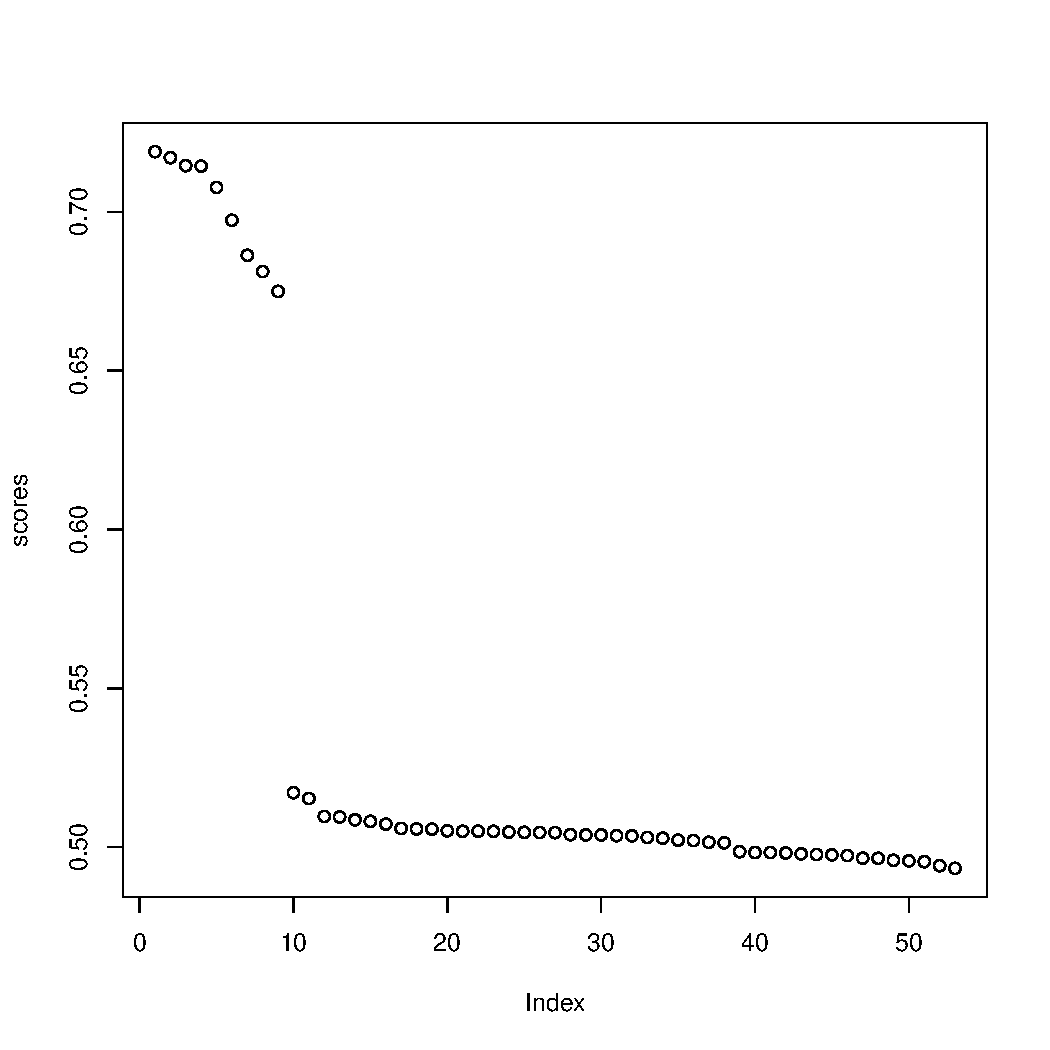
\includegraphics[width=\maxwidth]{figure/plotScores} 

\end{knitrout}

\newpage
\subsection{Plotting Maximum Common Substructure}
To calculate the MCSS for given clusters the function \Rfunction{getClusterMCSS} is used. This describes a 
a 1:1 atom correspondence between two compounds. The bond connection and atom types are equal
in both molecules in addition to the largest number of bonds or atoms. Such structural similarities
are often used to predict bioactive compounds \cite{Cao2008}.


\begin{knitrout}
\definecolor{shadecolor}{rgb}{0.969, 0.969, 0.969}\color{fgcolor}\begin{kframe}
\begin{alltt}
  \hlstd{clusterreps} \hlkwb{<-} \hlkwd{getClusterMCSS}\hlstd{(cluster,} \hlkwc{mols}\hlstd{=scoredMols,} \hlkwc{k}\hlstd{=}\hlnum{7}\hlstd{,} \hlkwc{which}\hlstd{=}\hlnum{1}\hlopt{:}\hlnum{7}\hlstd{)}
\end{alltt}
\end{kframe}
\end{knitrout}

Each MCSS of a cluster can be plotted separately - with an overlay of the 
cluster number with the function \Rfunction{plotMol}. This function requires i. a. molecules as IAtomContainer 
objects and an optional watermark (Figure \ref{fig:clusterep}). 
\begin{knitrout}
\definecolor{shadecolor}{rgb}{0.969, 0.969, 0.969}\color{fgcolor}\begin{kframe}
\begin{alltt}
  \hlkwd{plotMol}\hlstd{(clusterreps[[}\hlnum{1}\hlstd{]],} \hlkwc{watermark}\hlstd{=}\hlnum{1}\hlstd{)}
  \hlkwd{plotMol}\hlstd{(clusterreps[[}\hlnum{2}\hlstd{]],} \hlkwc{watermark}\hlstd{=}\hlnum{2}\hlstd{)}
  \hlstd{...}
\end{alltt}
\end{kframe}
\end{knitrout}


\setkeys{Gin}{width=0.3\textwidth}
\begin{figure}[h!]
\centering
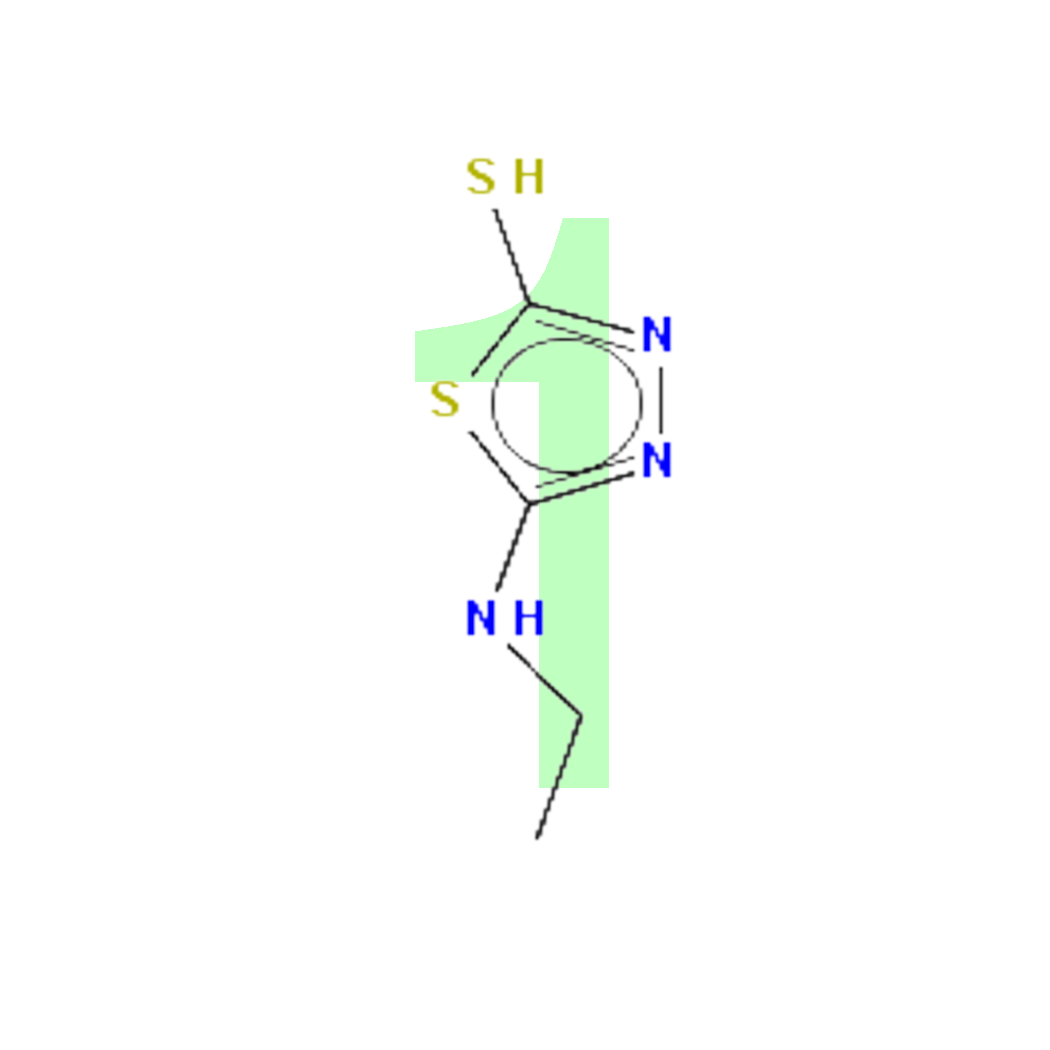
\includegraphics[width=0.25\textwidth]{./figure/plotClusterReps1.pdf}%
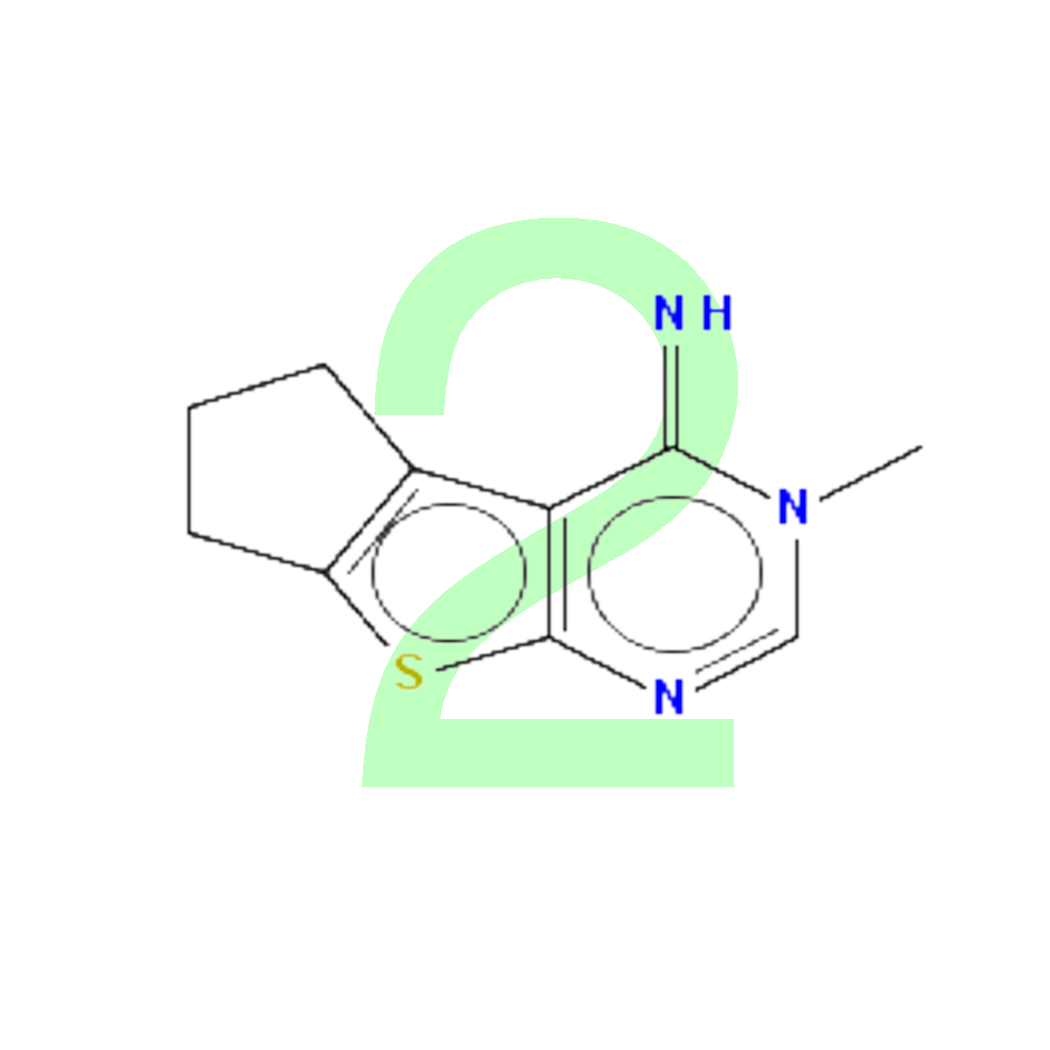
\includegraphics[width=0.25\textwidth]{./figure/plotClusterReps2.pdf}%
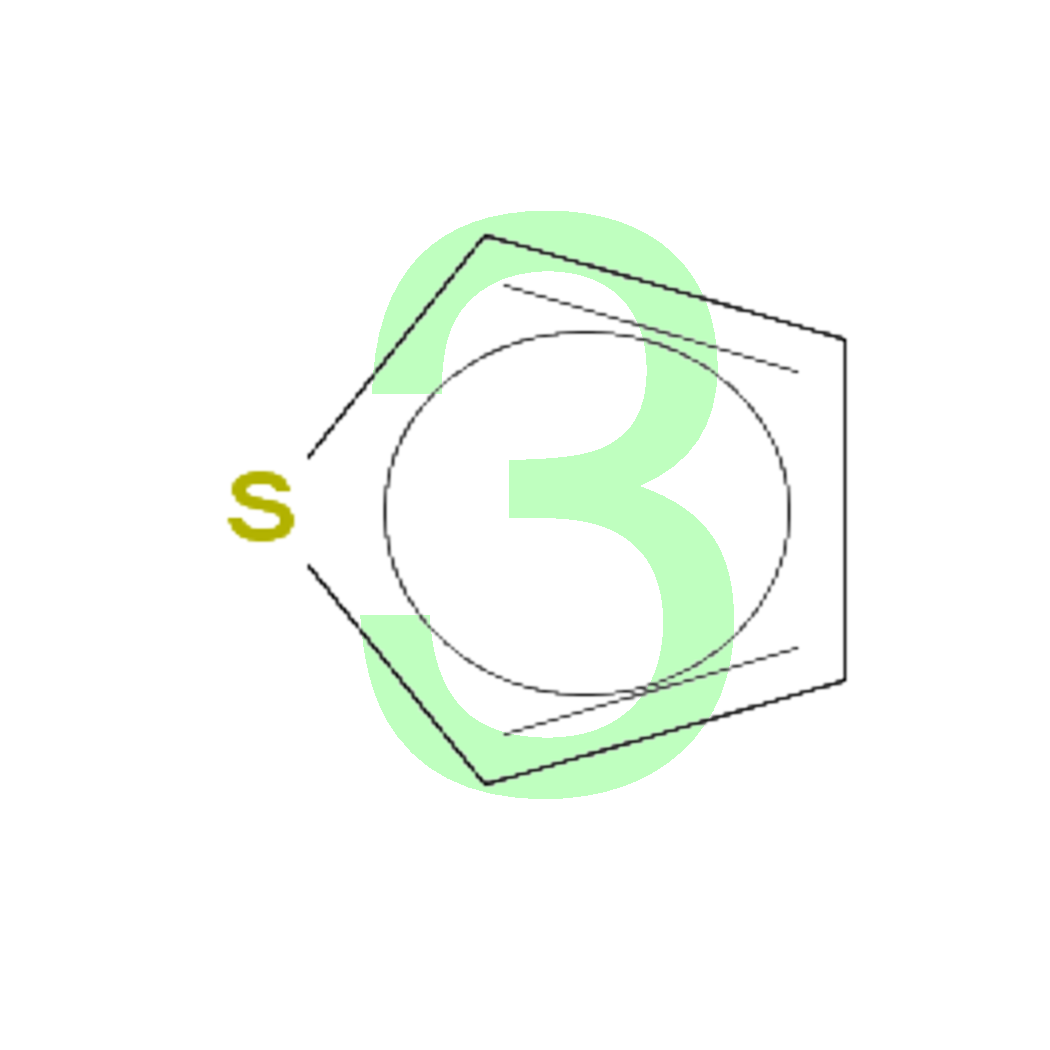
\includegraphics[width=0.25\textwidth]{./figure/plotClusterReps3.pdf}
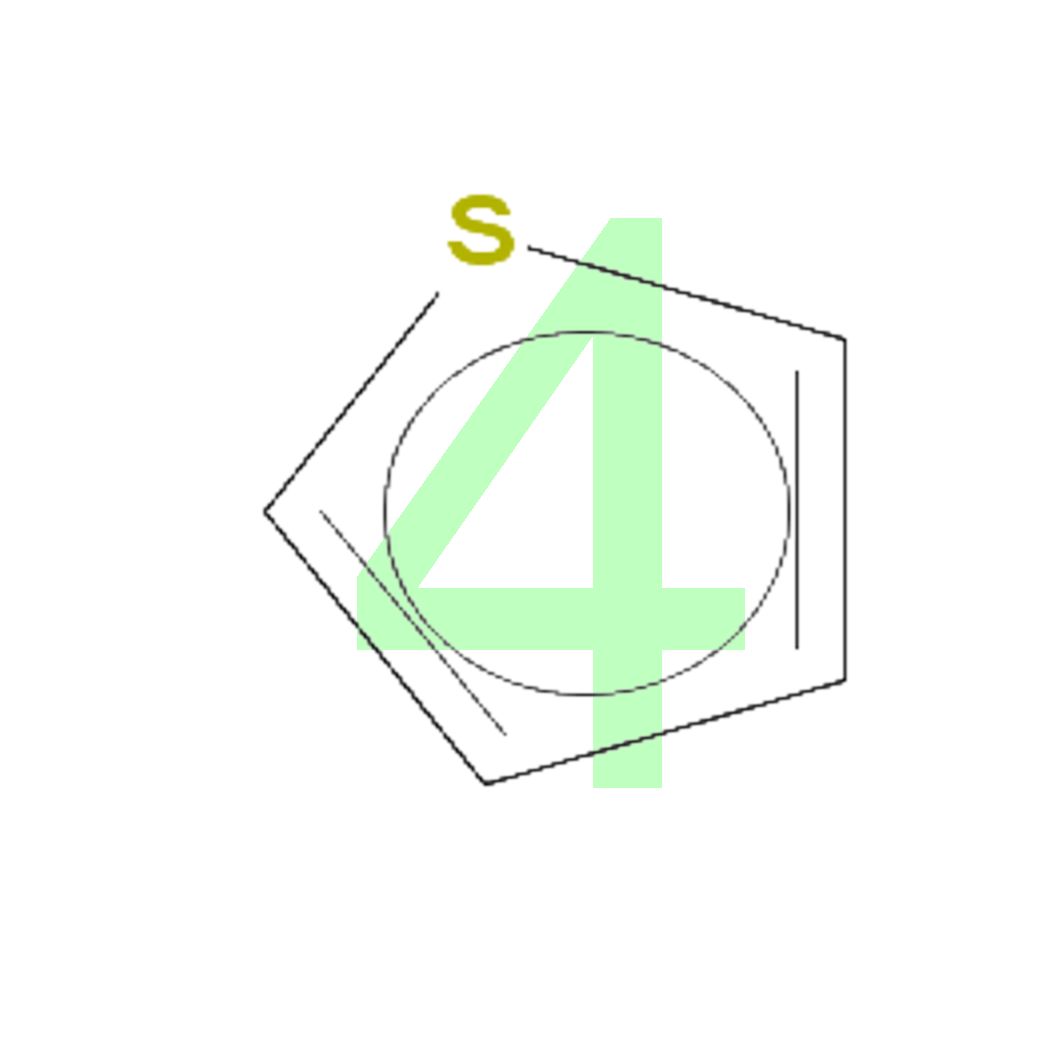
\includegraphics[width=0.25\textwidth]{./figure/plotClusterReps4.pdf}%

\includegraphics[width=0.25\textwidth]{./figure/plotClusterReps5.pdf}%

\includegraphics[width=0.25\textwidth]{./figure/plotClusterReps6.pdf}
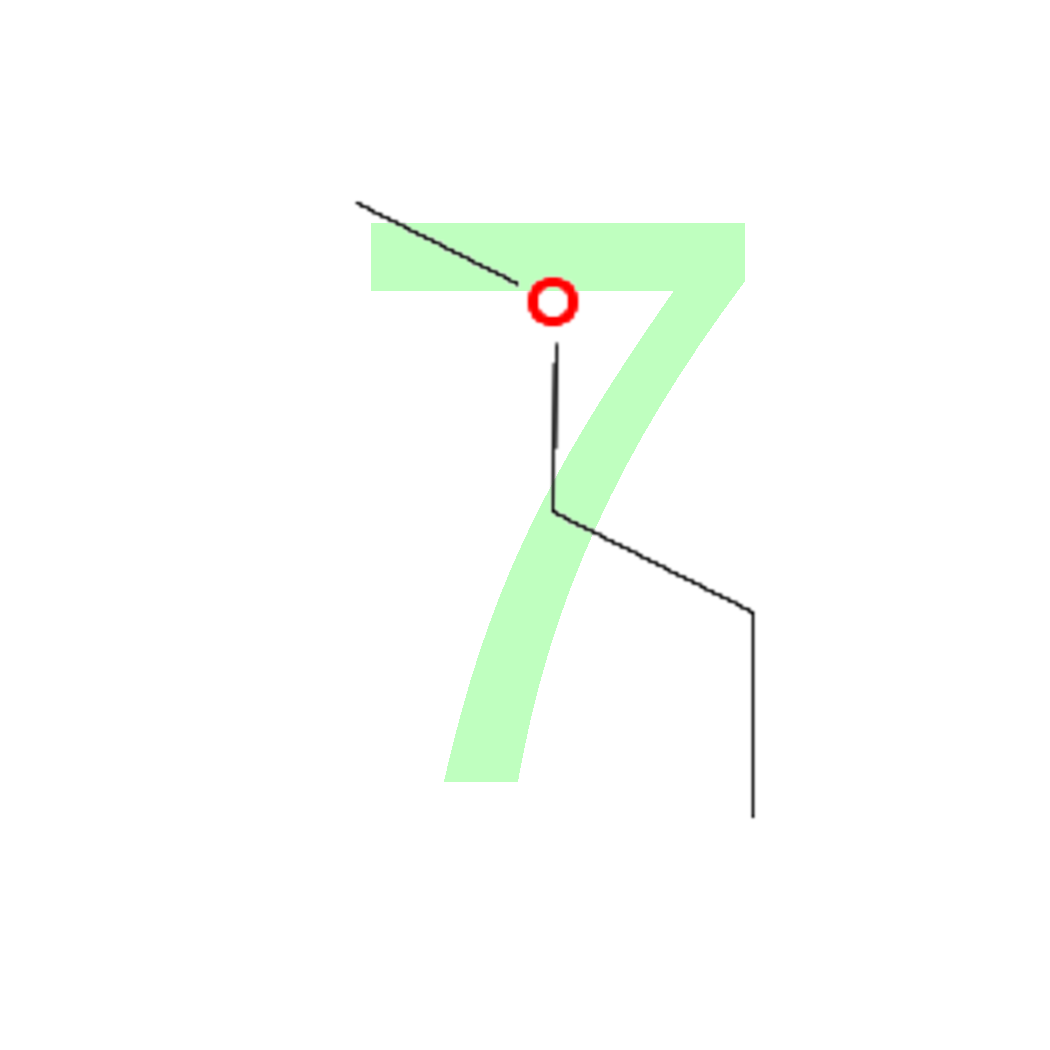
\includegraphics[width=0.25\textwidth]{./figure/plotClusterReps7.pdf}%
\caption{Plot of the most common substructure of each cluster with the number overlaid.}
\label{fig:clusterep}
\end{figure}
\setkeys{Gin}{width=0.8\textwidth}

\newpage
\subsection{Candidate Clustering}
\subsubsection{Clustering with displayed cluster numbers}
If we want to plot similar compounds in a dendrogram, firstly we have to create clusters. On that point we restrict the length of the list to the first 50 molecules and group them based on structural similarity. We could use a SD file or a list of compounds with the score property and the database property. In this example we get 10 groups.

\begin{knitrout}
\definecolor{shadecolor}{rgb}{0.969, 0.969, 0.969}\color{fgcolor}\begin{kframe}
\begin{alltt}
\hlstd{scoredMols} \hlkwb{<-} \hlstd{scoredMols[}\hlnum{1}\hlopt{:}\hlkwd{min}\hlstd{(}\hlnum{50}\hlstd{,} \hlkwd{length}\hlstd{(scoredMols))]}
\hlstd{cluster} \hlkwb{<-} \hlkwd{hclust.mols}\hlstd{(}\hlkwc{mols}\hlstd{=scoredMols,}
                       \hlkwc{scoreprop}\hlstd{=}\hlstr{"Score"}\hlstd{,}
                       \hlkwc{idprop}\hlstd{=}\hlstr{"DatabaseID"}\hlstd{)}
\end{alltt}
\end{kframe}
\end{knitrout}
To plot the molecule cluster as a dendrogram with cluster numbers overlaid, firstly we create a plot
either by applying \Rfunction{plot} or by using \Rfunction{hclust}. Then we create the numbers of each cluster.
For this purpose the maximum common substructure (MCSS) is calculated with $k=7$ clusters whereby all 7 
clusters are framed with a rectangle with a black border color. \\[0.5em]
Thereto, the clusters are drawn into the
consisting plot (Figure \ref{fig:plotNumDendro}). Hence, the height are referred as Tanimoto 
distance which formal formulated as \cite{Rogers1960}
\[
  T_d(X,Y) = -\log_2\left(\frac{\sum_i(X_i \land Y_i)}{\sum_i(X_I \lor Y_i)}\right)
\]
In our case, this describe the structural similarity of two different compounds to a third compound. 

\newpage
\begin{knitrout}
\definecolor{shadecolor}{rgb}{0.969, 0.969, 0.969}\color{fgcolor}\begin{kframe}
\begin{alltt}
\hlkwd{plot}\hlstd{(cluster,} \hlkwc{hang}\hlstd{=}\hlopt{-}\hlnum{1}\hlstd{)}
\hlkwd{myimages.clustNumbers}\hlstd{(cluster,} \hlkwc{k}\hlstd{=}\hlnum{7}\hlstd{,} \hlkwc{which}\hlstd{=}\hlnum{1}\hlopt{:}\hlnum{7}\hlstd{,} \hlkwc{border}\hlstd{=}\hlnum{2}\hlstd{)}
\end{alltt}
\end{kframe}\begin{figure}[h!]


{\centering 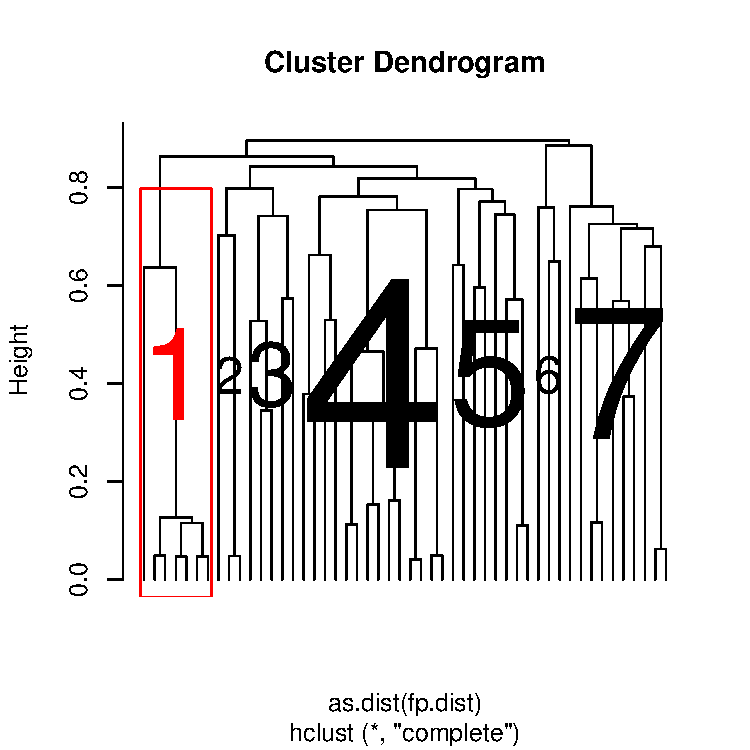
\includegraphics[width=\maxwidth]{figure/plotNumDendro} 

}

\caption[Example plot of clustered compounds]{Example plot of clustered compounds. If the MCSS is most similar two of 50 molecules joined into a single cluster illustrate by a vertical line. In contrast to that, if a cluster split into new cluster the horizontal bar illustrate the dissimilarity. The cluster can numbered and marked with a coloured border.\label{fig:plotNumDendro}}
\end{figure}


\end{knitrout}

\newpage
\subsubsection{Clustering with displayed MCSS}
If we want to plot the clusters with the most common substructure overlaid instead of a cluster
number, we create a cluster dendrogram as mentioned before. In the following, we use the function 
\Rfunction{myimages.hclust} to create MCSS below the cluster dendrogram (Figure \ref{fig:plotMCSSDendrogram}).

\begin{knitrout}
\definecolor{shadecolor}{rgb}{0.969, 0.969, 0.969}\color{fgcolor}\begin{kframe}
\begin{alltt}
\hlkwd{plot}\hlstd{(cluster,} \hlkwc{hang}\hlstd{=}\hlopt{-}\hlnum{1}\hlstd{)}
\hlkwd{myimages.hclust}\hlstd{(cluster,} \hlkwc{mols}\hlstd{=scoredMols,} \hlkwc{k}\hlstd{=}\hlnum{7}\hlstd{,} \hlkwc{which}\hlstd{=}\hlnum{1}\hlopt{:}\hlnum{7}\hlstd{,} \hlkwc{border}\hlstd{=}\hlnum{2}\hlstd{)}
\end{alltt}
\end{kframe}\begin{figure}[h!]


{\centering 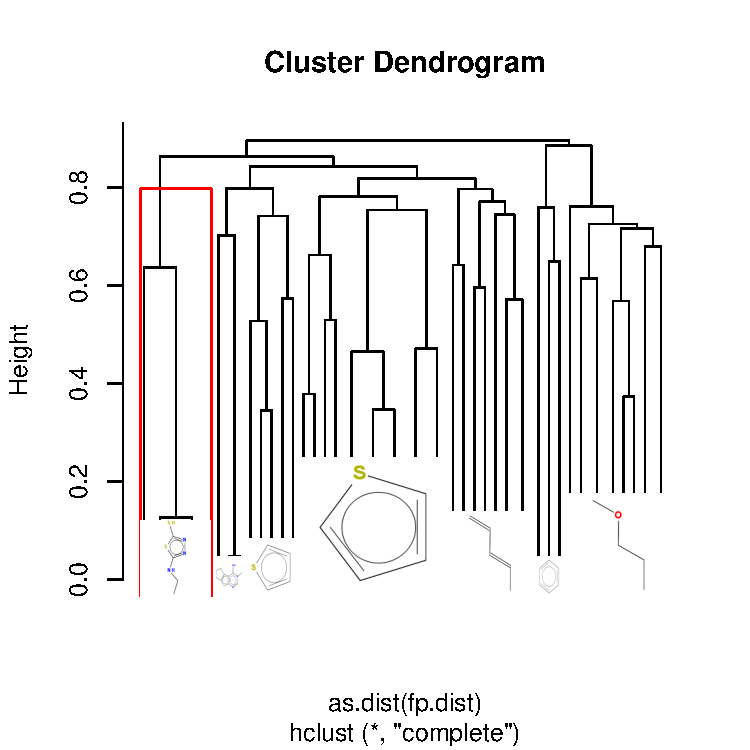
\includegraphics[width=\maxwidth]{figure/plotMCSSDendrogram} 

}

\caption[Cluster dendrogram of 50 sample compounds with given coloured border to mark a specific cluster]{Cluster dendrogram of 50 sample compounds with given coloured border to mark a specific cluster.\label{fig:plotMCSSDendrogram}}
\end{figure}


\end{knitrout}

\newpage
\subsubsection{Clustering with displayed Scores}
Instead of the MCSS or the cluster numbers we can plot the score and the color gradient, respectively.
Therefor, the function \Rfunction{plotCluster} is used. The function expects i. a. the list of the molecules
and the score which are listed in the properties of molecules.

\begin{knitrout}
\definecolor{shadecolor}{rgb}{0.969, 0.969, 0.969}\color{fgcolor}\begin{kframe}
\begin{alltt}
\hlkwd{plotCluster}\hlstd{(scoredMols,} \hlkwc{score}\hlstd{=}\hlstr{"Score"}\hlstd{,} \hlkwc{h}\hlstd{=}\hlnum{0.2}\hlstd{,} \hlkwc{scoreprop}\hlstd{=}\hlstr{"newscore"}\hlstd{)}
\end{alltt}
\end{kframe}
\end{knitrout}

The color indicates the level of a score of the compounds where a light red color indicates a high and a black
color a low score. Each compound contains a score which is plotted at the bottom of the figure as a red-black gradient. The height of the dendrogram is given as Tanimoto distance which is explained in section 3.3.1.

\begin{knitrout}
\definecolor{shadecolor}{rgb}{0.969, 0.969, 0.969}\color{fgcolor}

{\centering 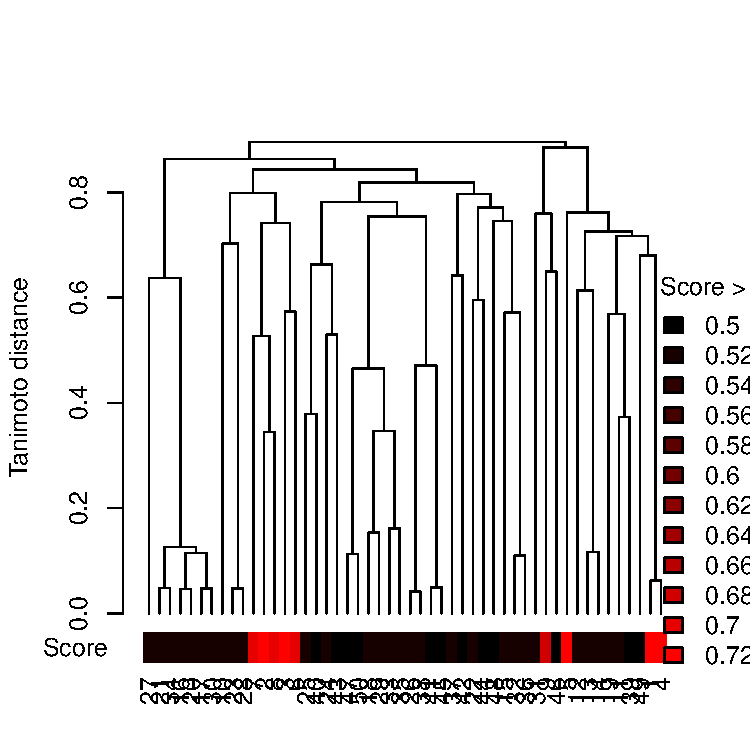
\includegraphics[width=\maxwidth]{figure/plotScoredDendrogram} 

}



\end{knitrout}

\newpage
\section{Summary}
In this manual the package 'metfRag' was described. Based on the precursor mass a candidate list of 
'KEGG' and 'PubChem' is returned. In future versions new databases will be added like 'ChemSpider'
or 'ChEMBL' to get more putative candidates. The databases especially 'PubChem' possess more several 
search methods whereby three methods are implemented. It is necessary to expand the 
capabilities to retrieve more accurate candidates, for example the combination of search methods per database.
\\[0.5em]
Several lists from different or the same databases can be processed by using simple set operations.
Thereto, the properties of the molecules are used which are returned. Nevertheless only sets with equal
properties are regared. To consider these compounds a homogenisation and preprocessing 
of the properties are necessary respectively. Hence, a thesaurus could applied to get the
suspected semantic synonyms of several property names while comparing the property names of 
each compound list. \\[0.5em]
The functionality of ranking is implemented. A scored compound list can be classified while 
numeric properties are used to rank the molecules to a specific order. Additionally the user
can write own functions which use molecule properties to calculate new values with which 
the ranking is determined. The optimistic and pessimistic rank as well 
as the relative rank can be calculated. \\[0.5em]
The scoring of a list of compounds performed by MetFrag which is written in Java and
integrated through \emph{rJava}.

\newpage
\printbibliography

\end{document}
